Ein Fahrzeug fährt auf einer geraden Strasse. Alle \SI{5}{\second} wird sein Ort $s$ gemessen:
\begin{center}
\begin{tabular}{l|ccccccc}
$t$ in \si{\second} & $0$ & $5$ & $10$ & $15$ & $20$ & $25$ & $30$ \\
\hline
$s$ in \si{\meter} & $-6$ & $-11$ & $-16$ & $-21$ & $-18$ & $-15$ & $-12$
\end{tabular}
\end{center}
\begin{abcliste}
\abc \DuSie{Zeichne}{Zeichnen Sie} das $s(t)$-Diagramm.
\abc \DuSie{Beschreibe}{Beschreiben Sie} die Bewegung in Worten: In welche Richtung und wie schnell fährt das Fahrzeug? Kehrt es um, und wenn ja, wann?
\abc Vier Schülerinnen und Schüler haben die Tabelle in ein Diagramm übertragen. Welches Diagramm ist richtig? Was wurde bei den anderen falsch gemacht?
\end{abcliste}
\begin{center}
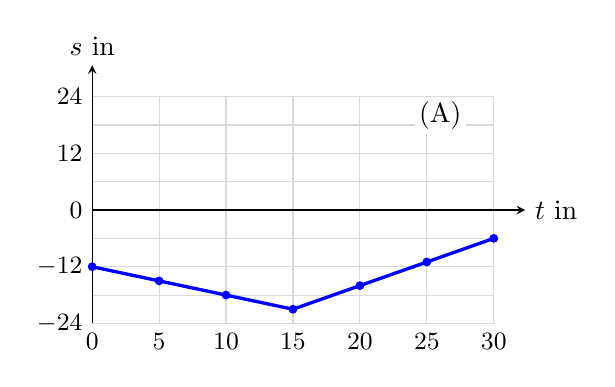
\begin{tikzpicture}[>=stealth, x=0.17cm, y=0.06cm]
 \draw[gray!30] (0,-24) grid[xstep=5, ystep=6] (30,24);
 \draw[->] (0,0) -- (32.353,0) node[right] {$t$ in \si{\second}};
 \draw[->] (0,-24) -- (0,30.667) node[above] {$s$ in \si{\meter}};
 \foreach \tk in {0,5,10,15,20,25,30} \node[below] at (\tk,-24) {\small $\tk$};
 \foreach \yk in {-24,-12,0,12,24} \node[left] at (0,\yk) {\small $\yk$};
 \draw[very thick, blue] (0,-12) -- (5,-15) -- (10,-18) -- (15,-21) -- (20,-16) -- (25,-11) -- (30,-6);
 \fill[blue] (0,-12) circle (1.6pt);
 \fill[blue] (5,-15) circle (1.6pt);
 \fill[blue] (10,-18) circle (1.6pt);
 \fill[blue] (15,-21) circle (1.6pt);
 \fill[blue] (20,-16) circle (1.6pt);
 \fill[blue] (25,-11) circle (1.6pt);
 \fill[blue] (30,-6) circle (1.6pt);
 \node[fill=white, inner sep=1.5pt] at (26,20) {(A)};
\end{tikzpicture}
\hspace{4mm}
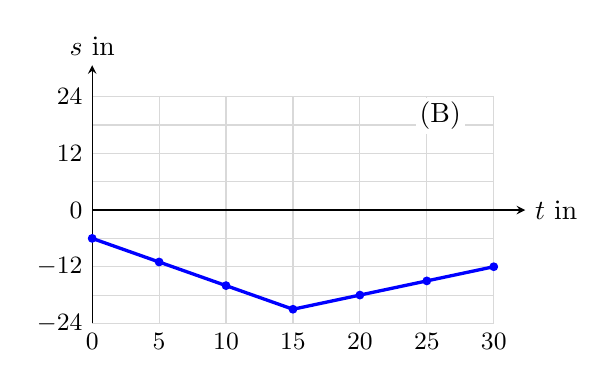
\begin{tikzpicture}[>=stealth, x=0.17cm, y=0.06cm]
 \draw[gray!30] (0,-24) grid[xstep=5, ystep=6] (30,24);
 \draw[->] (0,0) -- (32.353,0) node[right] {$t$ in \si{\second}};
 \draw[->] (0,-24) -- (0,30.667) node[above] {$s$ in \si{\meter}};
 \foreach \tk in {0,5,10,15,20,25,30} \node[below] at (\tk,-24) {\small $\tk$};
 \foreach \yk in {-24,-12,0,12,24} \node[left] at (0,\yk) {\small $\yk$};
 \draw[very thick, blue] (0,-6) -- (5,-11) -- (10,-16) -- (15,-21) -- (20,-18) -- (25,-15) -- (30,-12);
 \fill[blue] (0,-6) circle (1.6pt);
 \fill[blue] (5,-11) circle (1.6pt);
 \fill[blue] (10,-16) circle (1.6pt);
 \fill[blue] (15,-21) circle (1.6pt);
 \fill[blue] (20,-18) circle (1.6pt);
 \fill[blue] (25,-15) circle (1.6pt);
 \fill[blue] (30,-12) circle (1.6pt);
 \node[fill=white, inner sep=1.5pt] at (26,20) {(B)};
\end{tikzpicture}
\end{center}
\begin{center}
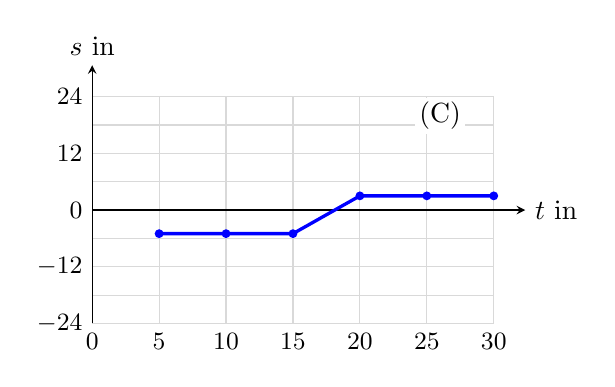
\begin{tikzpicture}[>=stealth, x=0.17cm, y=0.06cm]
 \draw[gray!30] (0,-24) grid[xstep=5, ystep=6] (30,24);
 \draw[->] (0,0) -- (32.353,0) node[right] {$t$ in \si{\second}};
 \draw[->] (0,-24) -- (0,30.667) node[above] {$s$ in \si{\meter}};
 \foreach \tk in {0,5,10,15,20,25,30} \node[below] at (\tk,-24) {\small $\tk$};
 \foreach \yk in {-24,-12,0,12,24} \node[left] at (0,\yk) {\small $\yk$};
 \draw[very thick, blue] (5,-5) -- (10,-5) -- (15,-5) -- (20,3) -- (25,3) -- (30,3);
 \fill[blue] (5,-5) circle (1.6pt);
 \fill[blue] (10,-5) circle (1.6pt);
 \fill[blue] (15,-5) circle (1.6pt);
 \fill[blue] (20,3) circle (1.6pt);
 \fill[blue] (25,3) circle (1.6pt);
 \fill[blue] (30,3) circle (1.6pt);
 \node[fill=white, inner sep=1.5pt] at (26,20) {(C)};
\end{tikzpicture}
\hspace{4mm}
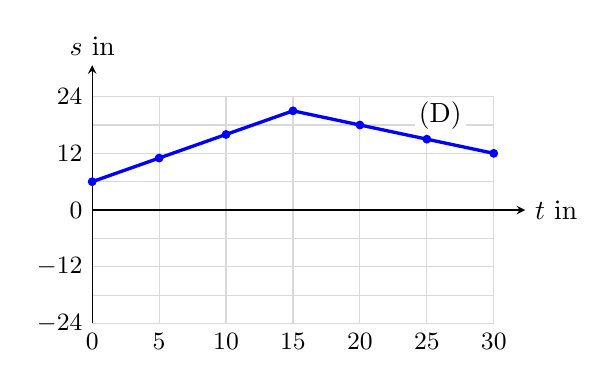
\begin{tikzpicture}[>=stealth, x=0.17cm, y=0.06cm]
 \draw[gray!30] (0,-24) grid[xstep=5, ystep=6] (30,24);
 \draw[->] (0,0) -- (32.353,0) node[right] {$t$ in \si{\second}};
 \draw[->] (0,-24) -- (0,30.667) node[above] {$s$ in \si{\meter}};
 \foreach \tk in {0,5,10,15,20,25,30} \node[below] at (\tk,-24) {\small $\tk$};
 \foreach \yk in {-24,-12,0,12,24} \node[left] at (0,\yk) {\small $\yk$};
 \draw[very thick, blue] (0,6) -- (5,11) -- (10,16) -- (15,21) -- (20,18) -- (25,15) -- (30,12);
 \fill[blue] (0,6) circle (1.6pt);
 \fill[blue] (5,11) circle (1.6pt);
 \fill[blue] (10,16) circle (1.6pt);
 \fill[blue] (15,21) circle (1.6pt);
 \fill[blue] (20,18) circle (1.6pt);
 \fill[blue] (25,15) circle (1.6pt);
 \fill[blue] (30,12) circle (1.6pt);
 \node[fill=white, inner sep=1.5pt] at (26,20) {(D)};
\end{tikzpicture}
\end{center}
